\documentclass[12pt,letterpaper]{article} % For LaTeX2e
\usepackage{amsmath,amsthm,amsfonts,amssymb,amscd}
\usepackage{booktabs}
% \usepackage[nofiglist, notablist]{endfloat}
\usepackage{fullpage}
\usepackage{graphicx}
\usepackage{lastpage}
\usepackage{listings}
\lstset{
	numbers=left,
	numbersep=5pt,
	stepnumber=1,
	tabsize=2,
	showstringspaces=false
}
\usepackage{enumerate}
\usepackage{fancyhdr}
\usepackage{final_project}
\usepackage{hyperref}
\usepackage{mathrsfs}
\usepackage{natbib}
\usepackage{cancel}
\usepackage{times}
\usepackage{tikz}
\usepackage{xcolor}
\usepackage[margin=3cm]{geometry}

% \renewcommand{\efloatseparator}{\mbox{}}




\title{A Social Choice Application}


\author{
Matt Dickenson\\
Department of Political Science\\
Duke University\\
Durham, NC 27708 \\
\texttt{mcd31@duke.edu}
}

\newcommand{\fix}{\marginpar{FIX}}
\newcommand{\new}{\marginpar{NEW}}

\nipsfinalcopy

\begin{document}

\begin{titlepage}

\clearpage
\maketitle
\thispagestyle{empty}

\begin{abstract}
This project implements a social choice web application, with an example use case of a group deciding on which movie to see. Using a formal voting process reduces the complexity of preference elicitation, prevents cascade effects arising from sequential preference revelation, and ensures privacy for voters, reducing the incentive for preference falsification. The Borda rule exhibits a number of desirable characteristics including anonymity, neutrality, unanimity, universal domain, and reinforcement. The major downside of Borda count is its manipulability; however, Monte Carlo simulations show that such manipulation should be rare in practice (especially with many voters) and that the decreases in average utility are relatively modest. Employing this application could greatly improve the coordination process for informal social gatherings. 
\end{abstract}

\end{titlepage}



\newpage

\section{Introduction}

\subsection{Motivation}

%What is the real-world problem your project will address? 

This project consists of three parts, centered around the implementation of a social choice web application. The application uses a formal voting process to reduce the complexity of preference elicitation. The Borda rule exhibits a number of desirable characteristics including anonymity, neutrality, unanimity, universal domain, and reinforcement. The major downside of Borda count is its manipulability. Monte Carlo simulations are used to assess the frequency and impact of such manipulations compared to the plurality and veto rules. 
These results suggest that manipulation should be rare in practice (especially with many voters) and have a modest impact on average utility. This suggests that employing the application's voting procedure could improve outcomes for coordinating group outings.

\subsection{Problem Definition} 

%Define this problem. What question are you trying to
%solve? What is the goal of the project?

The software application is intended to be used by a group coordinating on a single outcome by aggregating their preferences, e.g. selecting a movie for a night out with friends. A user creates a movie poll by supplying candidate options (movies) and voters (a list of email addresses to be contacted). A unique link is then sent to each voter, who supplies her ranking of the choices. When all votes have been recorded, an email is sent to all voters with the outcome (and possibly more info, such as anonymized rankings), and a link where they can indicate their satisfaction with the outcome. Using this application reduces the complexity of preference elicitation and avoids other undesirable issues that arise in informal group decision-making.


\section{A Social Choice Application}

\subsection{Voting Methods}

Desirable properties of the voting method for this application arise from both normative and pragmatic concerns. Anonymity and neutrality ensure that the names of the voters and candidates, respectively, do not influence the outcome. Candidates can be presented to voters in a randomized order to ensure that the format of the list does not bias results. Unanimity requires that if candidate $A$ is preferred over $B$ by all voters, $B$ should not win. The universal domain of potential ballots will be considered in the Monte Carlo simulations, to ensure that the application works with any opinion a voter might entertain about the candidates. Finally, we desire a rule with reinforcement, so that if disjoint sets of voters select the same winner, that candidate should win when the voters are pooled. Practically, this ensures that two small groups of friends who use the app and arrive at the same movie should also have seen that movie if they voted as a single group.

If there are two candidates, the only social decision method that satisfies neutrality, anonymity, and positive responsiveness (if a candidate is tied for the win and moves up in rankings, it will become the winner) is majority rule \citep{may1952}. Less strict conditions, such as Pareto optimality, also motivate the use of majority rule even if positive responsiveness is thought to be too strict \citep{acsan2002,j2003majority}. If there are more than two candidates, only a scoring rule will satisfy anonymity, neutrality, reinforcement, and continuity (if two subgroups of voters select different winners, then there is some number $k$ such that $k$ copies of the first subgroup plus a single copy of the second subgroup will elect the first group's winner) \citep{young1975}. Scoring rules have the additional advantage of being computationally easy.

What voting rule should we choose? Borda count chooses the majority alternative (whenever it exists), and satisfies anonymity, neutrality, unanimity, and reinforcement. A major downside of the Borda rule is that it is easily manipulable \citep{bartholdi1989computational}. However, for a particular type of manipulation (Constructive Coalitional Weighted-Manipulation), manipulating Borda is NP-complete for three candidates, and it is NP-hard for another manipulation (Constructive Individual Unweighted-Manipulation) under uncertainty about others' votes \citep{conitzer2007elections}. More than three candidates should be present for most use cases of the application proposed here. To assess the relative merits of using Borda in this application, Monte Carlo simulations will estimate its vulnerability to manipulation.

% conitzer2003universal
% conitzer2007elections
% xia2009complexity

\subsection{User Experience}

The application described above has been implemented using the Rails framework in the Ruby language. Although the application has not been deployed publicly, the screenshots in Figure \ref{example-screens} give a sense of the user experience. The basic usage process is as follows:
\begin{enumerate}
\item Upon arriving at the homepage, a user is invited to create a poll by supplying candidate options (movie-showtime-location tuples drawn from the Fandango API--see the left pane of Figure \ref{example-screens})
\item The user then invites voters by supplying their names and email addresses
\item An email is sent to each voter inviting her to participate in the poll
\item If the voter chooses to cast a vote, she clicks the unique link in the email (to avoid the need for remembering the password for a user account) and is taken to the voting page (right pane of Figure \ref{example-screens})
\item When all votes are recorded or a deadline has been reached (minimum of one hour before the first canddiate showtime), an email is sent to all voters with the outcome
\end{enumerate}


\begin{figure}[h!]
 \begin{center}
  \begin{minipage}{0.45\textwidth}
    \begin{center}
      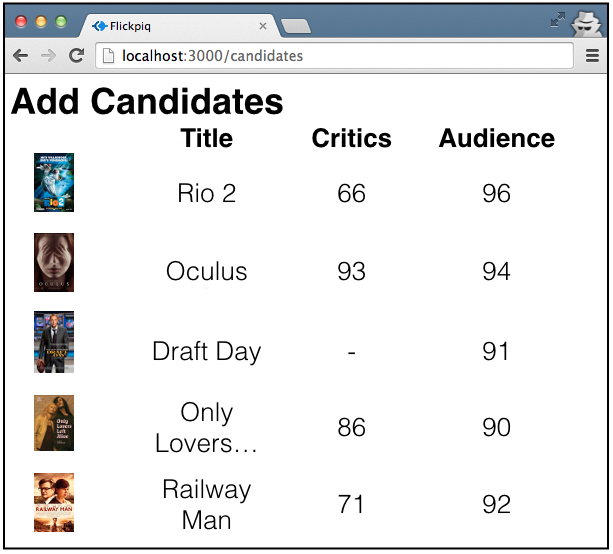
\includegraphics[scale=0.25]{../graphics/add-candidates.png}
    \end{center}
  \end{minipage}
  \hspace{0.05\textwidth}
  \begin{minipage}{0.45\textwidth}
    \begin{center}
      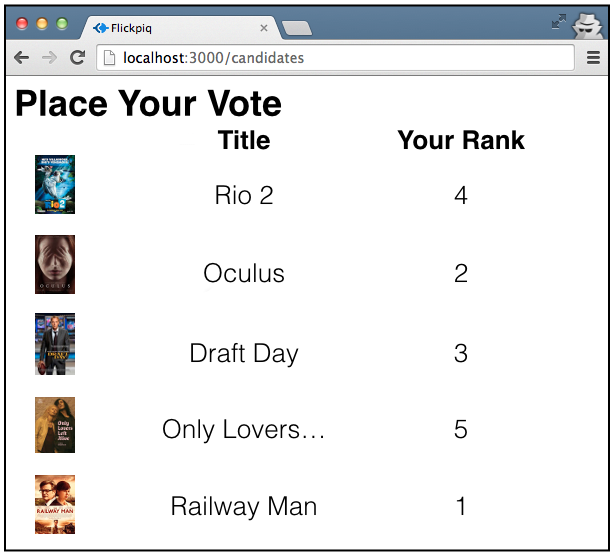
\includegraphics[scale=0.25]{../graphics/place-vote.png}
    \end{center}
  \end{minipage} \\
  \caption{Example screens for poll creator to add candidate movies (left) and for voter to rank movies (right).}
  \label{example-screens}
 \end{center}
\end{figure}



\subsection{Complexity of Elicitation}

How does using this application improve the process of selecting a movie for a group outing? One advantage of this method is that it reduces the average complexity of preference elicitation. When a group coordinates directly over email, there are several disadvantages. First, the pool of voters is not pre-defined: anyone could be added to or omitted from the email conversation at any time. Second, the domain of candidates is not fixed: a new candidate could be added at any time (even when the group is nearing a consensus), extending the time to elicitation exponentially. Third, preferences are expressed in sequence, leading to potential cascading effects resulting in suboptimal outcomes. Fourth, because preferences are not expressed privately voters may feel pressure to engage in preference falsification.
% todo: cite literature on cascading/herd behavior

The use of a voting application overcomes each of these disadvantages. The number of messages needed in a traditional email exchange is combinatorial in the number of voters, $n$, and candidates, $m$. the number of email messages sent by the voting application is $O(n)$: one message for each voter to request her vote, and one message to each voter to reveal the outcome.


\section{Simulation and Analysis}

This application reduces the complexity of preference elicitatation (as described above), but how vulnerable is it to manipulation? Manipulability is a known weakness of the Borda voting method. To assess the risk of manipulation in this application, simulations were conducted to compare Borda count to the plurality and veto rules. 

\subsection{Manipulation Method}

The manipulation method explored is a utility-maximizing variant of the Find-Two-Winners (FTW) manipulation. The version employed in this paper is unweighted (all votes have weight $w=1$) and there is a single potential manipulator. The manipulator $M$ calculates a strategic vote as follows:
\begin{enumerate}
\item Let $v_M$ denote $M$'s vote, initialized to be her true ranked preferences.
\item Run the voting rule with $v_M$ and all other voter's true votes (or an estimate of their votes, if simulating without perfect information). Let the winner of this vote be denoted $c_1$.
\item For every other candidate $c_2 \neq c_1$:
  \begin{itemize}
    \item Let $\hat{v}_{M,c_2}$ be a vote in which $M$ ranks $c_2$ first and $c_1$ last (leaving all other rankings unchanged)
    \item Run the voting rule with $\hat{v}_{M,c_2}$ replacing $M$'s true preferences, leaving all other votes unchanged. Denote the winner of this vote $c$.
    \item If $U_M(c) > U(c_1)$, let $v_M=\hat{v}_{M,c_2}$.
  \end{itemize}
\item Return $v_M$
\end{enumerate}
% todo: cite conitzer on find two winners: non-existence of voting rules that are usually hard to manipulate...


\subsection{Simulation Parameters}

Voting was simulated with three different rules: Borda count, plurality, and veto. In addition to the manipulation method, a number of additional simulation parameters were used to model the voting process. Movies, $m$, were treated as having two distinct attributes that influence utility: a critic rating, $r_c$, and an audience rating, $r_a$ (both expressed as a percentage). Voters, $v$, differ in the weights, $w$, that they assign to critics' ratings, so that $U_{v_i}(m_j) = w(r_c(m_j)) + (1-w)(r_a(m_j))$ The four movies used for the simulations had audience and critic ratings of $(0.00, 0.60), (0.45, 0.45), (0.70, 0.20)$, and $(0.77, 0.20)$. Although somewhat unrealistic as ratings for actual movies, these values were chosen so that each movie would be ranked first over one-fourth of the range of $w$ (see Figure \ref{fake-utils}).

\begin{figure}
\begin{center}
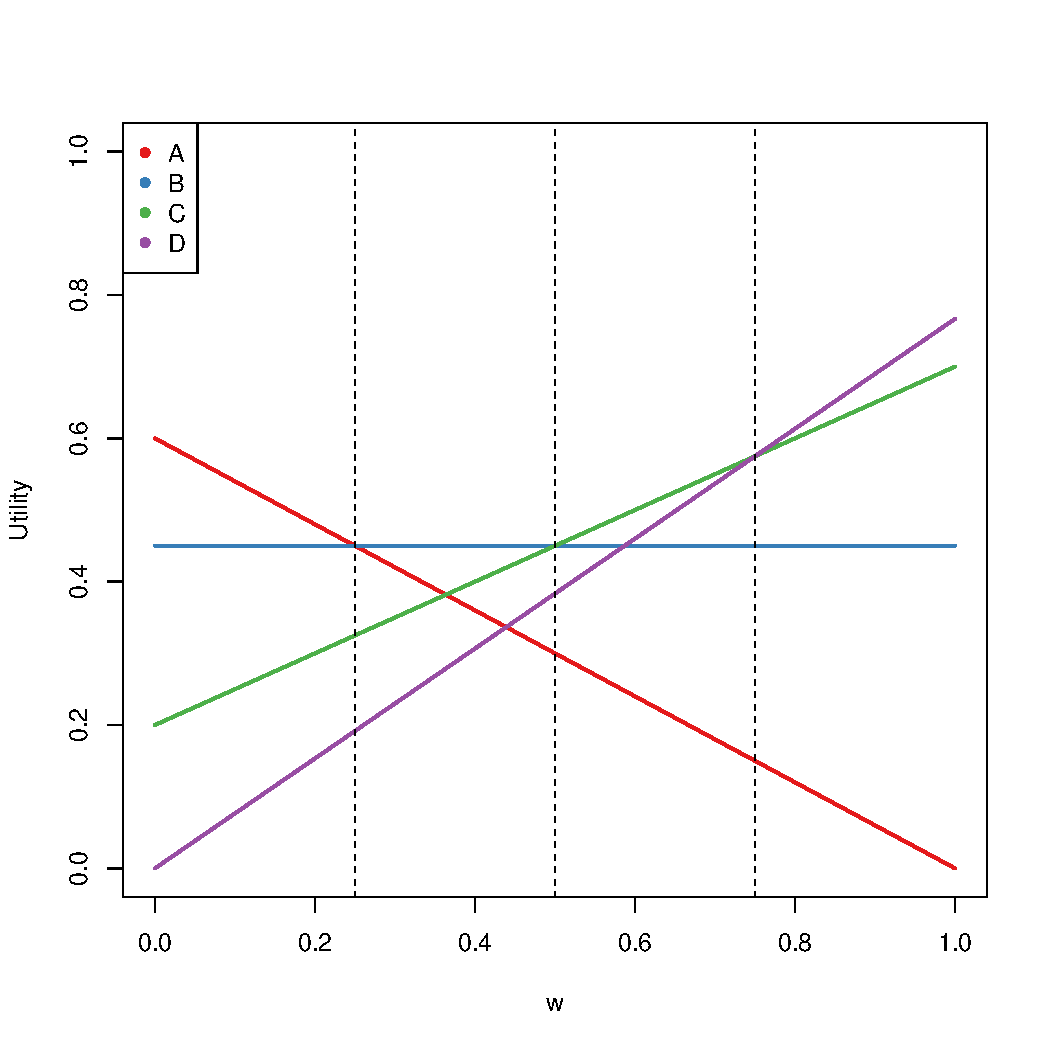
\includegraphics[scale=0.4]{../graphics/fakeUtils.pdf}
\caption{A voter's utility for four example movies as a function of $w$. Dashed lines indicate changes in the first-ranked candidate.}
\label{fake-utils}
\end{center}
\end{figure}

Voters' weights were sampled from the Beta distribution with parameters $(\alpha, \beta) = \{ (9,1), (7,3), (5,5), (3,7), (1,9) \}$. This allows the mean of $w$ to vary from 0.1 to 0.9 by increments of 0.1. The manipulator's weight values varied along the same range, but were drawn independently of the voters'. In half of simulations the manipulator knew the other voters' weights exactly, and in the other half she had to estimate them by maximum likelihood from the common prior (i.e. $\alpha$ and $\beta$ were known to the manipulator). The number of non-manipulating voters was varied from one to 10. 100 simulations were run for each combination of these parameters.




\subsection{Frequency of Manipulation}

How frequently was manipulation observed in the simulations? Overall, manipulation occurred in 18.7 percent of simulations using the Borda rule, 2.1 percent of simulations using plurality, and 80 percent of simulations with the veto rule. For both Borda and plurality, manipulation was observed less often under imperfect information (see Table \ref{table:frequencies}). For these two rules the rate of manipulation decreases in the number of non-manipulating voters, and the difference between them is negligible with eight or more non-manipulators voting (see Figure \ref{manipulation-frequency}. In reality the manipulator will have imperfect information about others' votes, suggesting that actual manipulations with this application will be uncommon. 

\begin{table}[h!]
\begin{center}
\caption{Frequency of Manipulation by Voting Rule}
\label{table:frequencies}
\begin{tabular}{lcc}
\multicolumn{1}{c}{} & \multicolumn{1}{c}{Perfect Information} & \multicolumn{1}{c}{Imperfect Information} \\
\hline
Borda     & .20 & .17 \\
Plurality & .03 & .01 \\
Veto      & .80 & .80 \\
\end{tabular}
\end{center}
\end{table}


\begin{figure}[h!]
\begin{center}
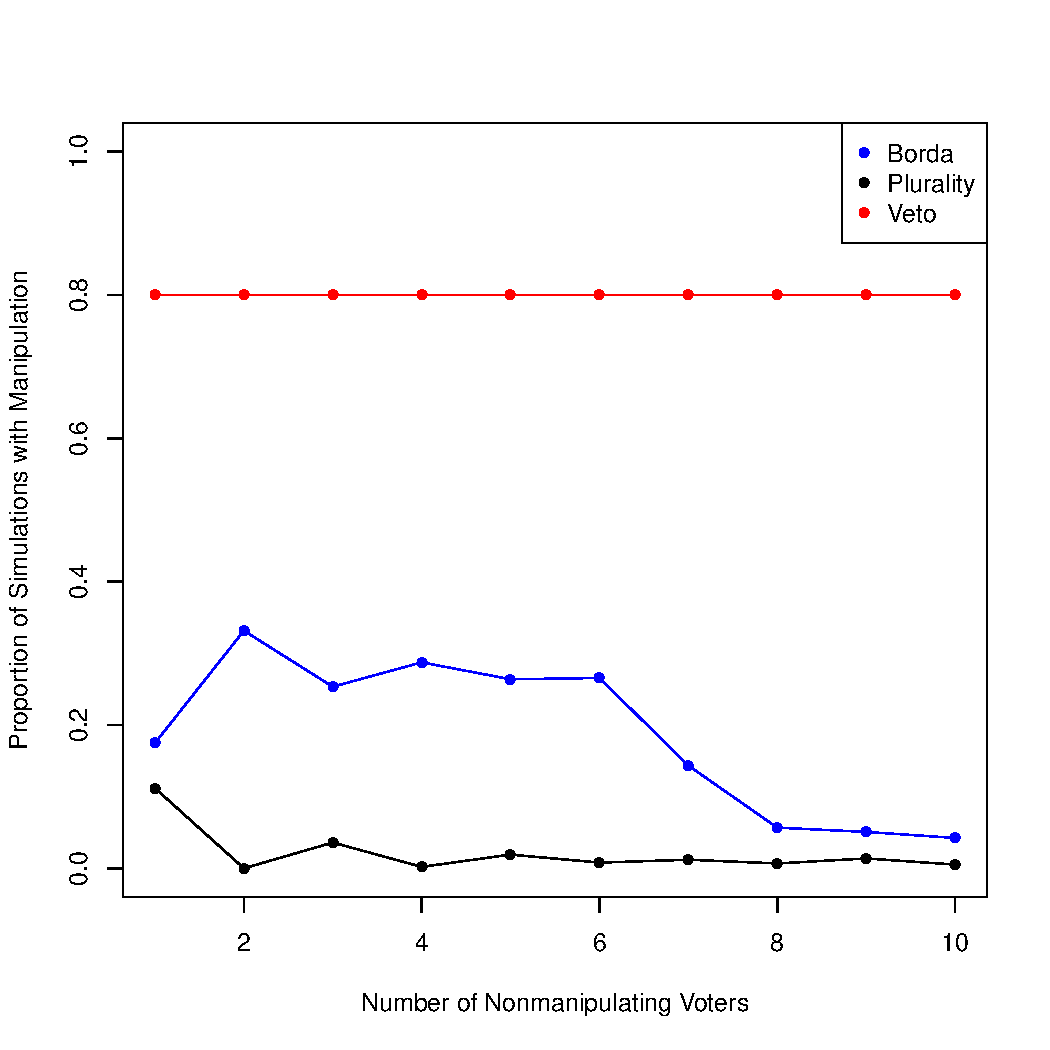
\includegraphics[scale=0.4]{../graphics/manipulation-frequency.pdf}
\caption{Observed frequency of manipulation by voting rule and number of non-manipulating voters.}
\label{manipulation-frequency}
\end{center}
\end{figure}

\subsection{Utility With and Without Manipulation}

How do voters fare under each of the three voting rules? Unsurprisingly, non-manipulators have lower average utility when manipulation occurs (Table \ref{table:utilities}). Manipulators do better on average when their manipulation is successful (unsurprisingly, since the manipulation attempt is utility-maximizing) except under the veto rule. Although this is odd, further inspection revealed that the average under manipulation with the veto rule was being pulled down by a few outliers, while the maximum with manipulation was much higher (again, for the manipulator) than without. Histograms for the observed utility distributions in 50,000 simulations with the Borda count rule are shown in Figure \ref{nonmanip-manip-utils}. The modest decrease in average utility observed under manipulation, accompanied by the relative infrequency of manipulation, suggest that the Borda rule is acceptable for this application. 

\begin{center}
\begin{table}
\caption{Average utilities by scenario}
\label{table:utilities}
\begin{tabular}{lcccc}
\multicolumn{1}{c}{} & \multicolumn{2}{c}{Manipulator} & \multicolumn{2}{c}{Nonmanipulator} \\
\multicolumn{1}{c}{} & With Manipulation & Without Manipulaiton & With Manipulation & Without Manipulaiton \\
\hline
Borda     & .58 & .44 & .43 & .76 \\
Plurality & .55 & .44 & .40 & .72 \\
Veto      & .51 & .55 & .60 & .62 % weird, but higher max w/manip
\end{tabular}
\end{table}
\end{center}

\begin{center}
\begin{figure}[h!]
\begin{minipage}{0.45\textwidth}
\begin{center}
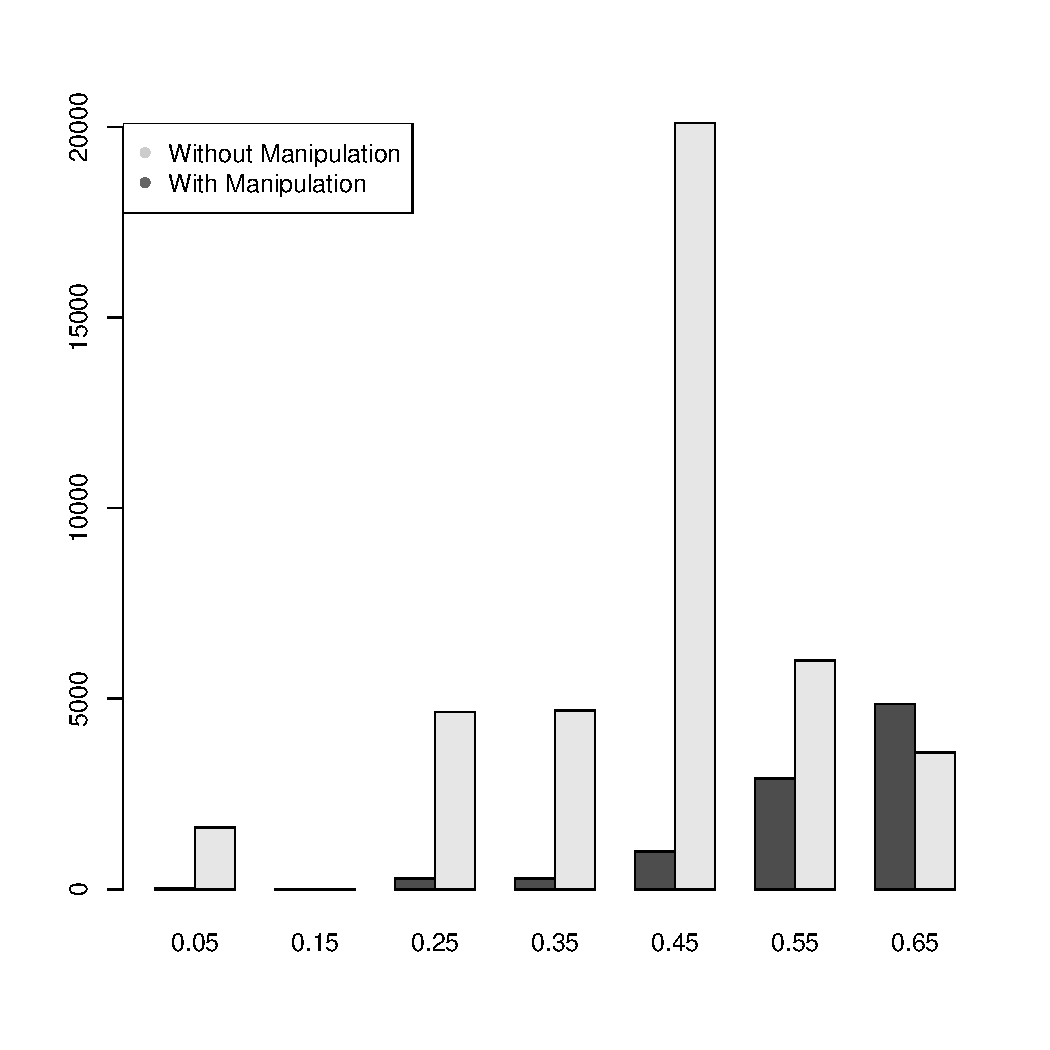
\includegraphics[scale=0.4]{../graphics/manipulator-utilities.pdf}
\end{center}
\end{minipage}
\hspace{0.05\textwidth}
\begin{minipage}{0.45\textwidth}
\begin{center}
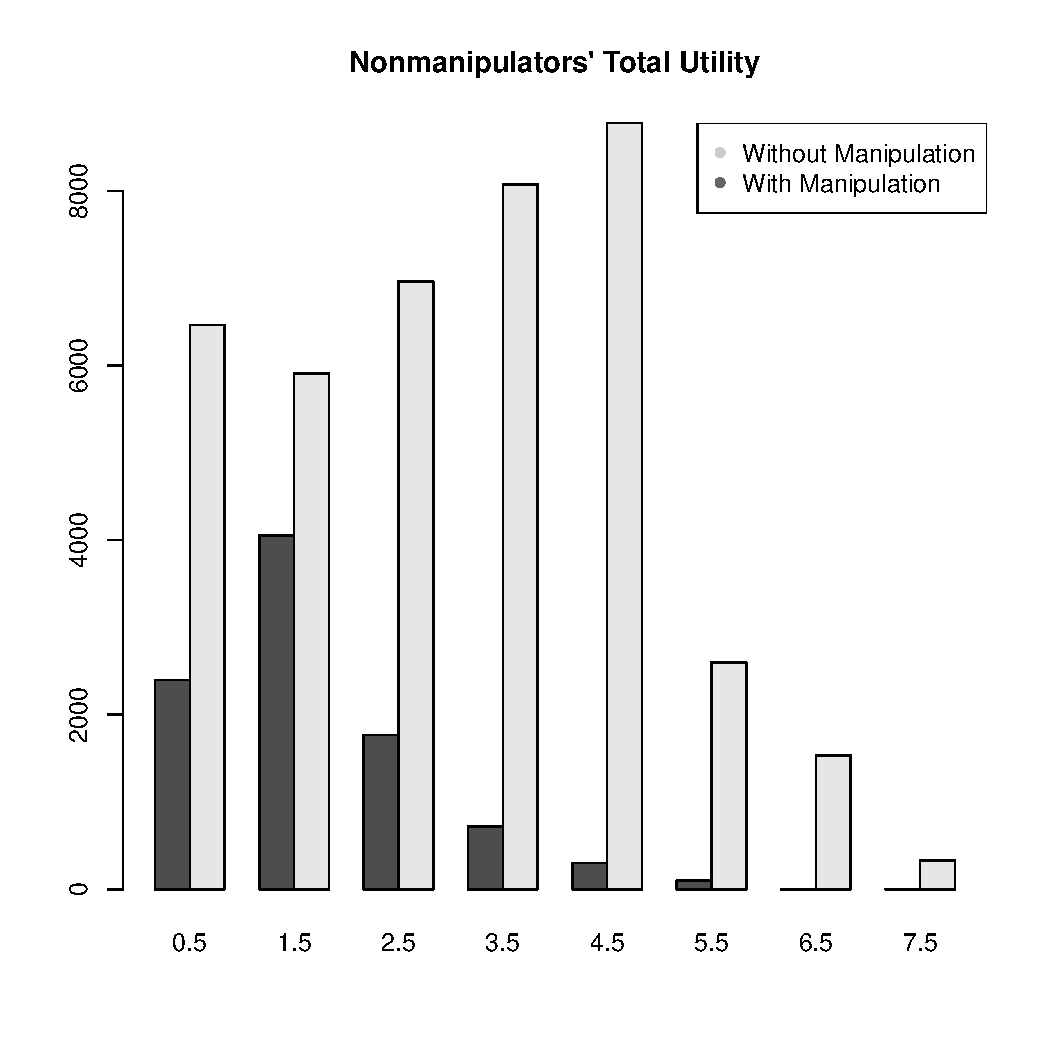
\includegraphics[scale=0.4]{../graphics/nonmanipulators-utilities.pdf}
\end{center}
\end{minipage}
\caption{Manipulator's utility distribution (left) and nonmanipulators' average utility distribution (right) with and without manipulation for Borda count simulations.}
\label{nonmanip-manip-utils}
\end{figure}
\end{center}


% \section{Related Work}

\section{Discussion} 

There are several promising avenues for further research on this project. A more sophisticated simulation model could consider a prior stage in which the poll organizer selects candidates from a larger pool of options, and assess the effect that this has on the outcome. The voting rule could also be left up to the participants by asking which criteria are desired for a particular situation. Instead of voting an auction could be used so that group members split the cost of the outing, with lower costs for those who dislike the outcome (setting a minimum threshold ensures that the outing occurs only if enough revenue is raised to pay for it). A more sophisticated model of movie-going would account for the combinatorial nature of movies--as combinations of showtimes, films, and locations--and allow voters to express preferences over each of these features separately. This would allow, for example, voters who feel strongly about the time of day but care less about what film they view to have their preferences taken into account. 

Implementing a web application in which users can employ Borda voting to coordinate a group decision extends the use of social choice to a popular setting. Using a formal voting process reduces the complexity of preference elicitation, prevents cascade effects arising from sequential preference revelation, and ensures privacy for voters, reducing the incentive for preference falsification. The Borda rule exhibits a number of desiragle characteristics including anonymity, neutrality, unanimity, universal domain, and reinforcement. The major downside of Borda count is its manipulability; however, Monte Carlo simulations showed that we should expect such manipulation to be rare in practice (especially with many voters) and that the decreases in average utility are relatively modest. Employing this application could greatly improve the coordination process for informal social gatherings. 

% take into account combinatorial nature of movie-showtime-location



\subsubsection*{Acknowledgments}

Thanks to Vincent Conitzer and course participants for feedback on earlier versions of this project. Any conclusions or errors are the sole responsibility of the author.

\subsubsection*{References}

% CITE A LOT. Any unreferenced methods, prior work, or biological phenomenon, unless it is textbook-common, will be penalized.


\begingroup
\renewcommand{\section}[2]{}
\bibliographystyle{unsrt}
\bibliography{/Users/mcdickenson/Documents/Templates/RefLib.bib}
\endgroup

\end{document}
